% ============================================================
%  BehaviorGuard — IEEE conference submission
%  Compile:   pdflatex → pdflatex × 2
% ============================================================
\documentclass[conference]{IEEEtran}

% ── Packages ─────────────────────────────────────────────────
\usepackage{microtype}
\usepackage{amsmath,amssymb}
\usepackage{graphicx}
\usepackage{booktabs}
\usepackage{multirow}
\usepackage{xcolor}
\usepackage{hyperref}
\usepackage{cleveref}
\usepackage{algorithm}
\usepackage{algpseudocode}
\usepackage{caption}
\usepackage{subcaption}
\usepackage{enumitem}
\usepackage{url}

% ── Hyperref colours ─────────────────────────────────────────
\hypersetup{
  colorlinks=true,
  linkcolor=blue!60!black,
  citecolor=green!50!black,
  urlcolor=blue!70!black,
}

% ── Convenience macros ───────────────────────────────────────
\newcommand{\BG}{\textsc{BehaviorGuard}}
\newcommand{\seman}{s_{\mathrm{sem}}}
\newcommand{\ling}{s_{\mathrm{ling}}}
\newcommand{\temp}{s_{\mathrm{temp}}}
\newcommand{\anomaly}{s_{\mathrm{anom}}}
\newcommand{\Pu}{P_u}
\newcommand{\munew}{\mathbf{m}_{\mathrm{new}}}
\newcommand{\eu}{\boldsymbol{\mu}_u}
\newcommand{\ew}{\mathbf{e}}
\definecolor{highF1}{RGB}{0,128,0}
\definecolor{lowF1}{RGB}{180,0,0}


% ============================================================
\begin{document}
% ============================================================

\title{\textbf{\BG}: Context-Aware Anomaly Detection\\
       in Conversational AI via Behavioral User Profiling}

\author{%
\IEEEauthorblockN{Dinmukhammed Mynzhassar\IEEEauthorrefmark{1}}
\IEEEauthorblockA{%
  \textit{Independent Research}\\
  Astana, Kazakhstan\\
  mynzhasardimash@gmail.com\\
  \IEEEauthorrefmark{1}\url{https://github.com/Va11eyard/BehaviorGuard}}
}
\maketitle

% ── Abstract ─────────────────────────────────────────────────
\begin{abstract}
Large language models deployed in conversational systems face a class of threats that
content-based safety mechanisms cannot adequately address: multi-turn request sequences
that appear benign in isolation yet pursue account takeover, credential harvesting, or
social engineering when aggregated across a user's interaction history.
Recent autonomous offensive AI systems demonstrate that adversarial intent can be
distributed across individually innocuous conversational turns, evading per-request
content filters.

We introduce \BG{}, to our knowledge the first system adapting behavioral profiling
methods (UEBA-style online baselines) to conversational-LLM anomaly detection with
emphasis on sequential detection.
\BG{} profiles each user via exponential moving average (EMA) embedding centroids,
online linguistic statistics, and temporal session patterns; it operates at the
embedding layer without modifying model weights or requiring LLM inference at
detection time, and routes flagged requests through tiered response policies driven
by a learned composite of semantic, linguistic, and temporal deviation scores.

A first-pass evaluation on three conversational benchmarks---PersonaChat, Blended
Skill Talk, and Anthropic HH---augmented with injected adversarial sequences
suggested strong per-message performance (F1 of 0.693, 0.794, and 0.642 at a fixed
threshold, overrides disabled).
Re-evaluation at realistic anomaly prevalence, however, shows that these figures are
an artifact of positive-enriched sampling: on the full PersonaChat holdout
(10{,}165 messages, 29 positives, 0.29\% prevalence) the same configuration collapses
to F1 $= 0.0059$ with a 90.5\% false-positive rate.
We analyze this \emph{base-rate evaluation artifact}---linguistic-score saturation
pushes 90.5\% of benign messages over the fixed threshold, which is invisible at
48\% sample prevalence but catastrophic at realistic base rates---and argue that
fixed-threshold F1 on enriched samples should not be reported for rare-event
detectors.

We then show that the underlying behavioral signal is real but too weak for
per-message thresholding, and that it is recovered by \emph{sequential accumulation}:
a CUSUM statistic over per-user embedding residuals detects mid-conversation author
substitution (an account-takeover proxy) with AUC 0.974 and 63.0\% episode detection
at a false-alarm budget of 1 per 1{,}000 benign messages on PersonaChat (median delay
4 messages), and AUC 0.900 with 35.0\% detection on Blended Skill Talk, where the
degradation quantifies PersonaChat's persona-conditioning advantage.
A length-matched placebo control (null detection 0.7\% and 0.1\% respectively)
confirms the signal is authorship change, not a stream-length artifact.
Per-message detectors---including \BG{}'s own composite---detect at most 1.3\% of the
same episodes at the same false-alarm budget.

The contribution of this paper is therefore twofold: a diagnosed evaluation
methodology failure that we believe is common in sparse behavioral anomaly detection,
and evidence across two datasets, with a null-hypothesis control, that
cross-session behavioral security should be framed as sequential (episode-level)
detection rather than per-message classification.
Validation on real-world adversarial corpora remains future work.
\end{abstract}

\begin{IEEEkeywords}
behavioral anomaly detection, conversational AI, LLM security, user profiling, account takeover, EMA embeddings
\end{IEEEkeywords}

% ── Table of Contents (remove for camera-ready) ─────────────
% \tableofcontents\newpage

% ============================================================
\section{Introduction}
\label{sec:intro}
% ============================================================

When a user who has spent months asking about Python debugging and API design suddenly
issues a request to ``delete all accounts, export all financial records, and disable
two-factor authentication'', should the conversational AI respond normally?
In today's deployed systems, the answer is usually yes---provided no individual request
explicitly violates a content-safety policy.
This is not an edge case.
It is the attack surface exploited by documented campaigns in which commercial LLMs
were used as autonomous offensive agents~\cite{anthropic2025espionage}, and more
recently by systems such as Claude Mythos, which demonstrated autonomous multi-step
vulnerability chaining across sessions~\cite{anthropic2026mythos}.
Project Glasswing subsequently gave $\sim$150 defender organizations access to Mythos
capabilities and surfaced over 10{,}000 high- or critical-severity vulnerabilities,
establishing that offensive AI tooling now outpaces defensive monitoring at
organizational scale~\cite{anthropic2026glasswing}.

Existing safeguards for LLM-based conversational systems focus on classifying the
\emph{content} of individual prompts and completions.
Llama Guard~\cite{inan2023llamaguard,meta2024llamaguard3} applies a fixed hazard
taxonomy to each request independently.
Constitutional AI~\cite{bai2022constitutional} and Safe RLHF~\cite{dai2023saferlhf}
embed normative constraints at training time.
These approaches reduce overtly harmful content, but they share a structural blindspot:
they evaluate each message in isolation, without knowledge of \emph{who} is sending it
or whether the message is anomalous relative to that user's established behavioral
baseline.
DARPA's AI Cyber Challenge (AIxCC), which concluded in August 2025, confirmed that AI
systems can autonomously find and patch software vulnerabilities at competition
scale~\cite{darpa2025aixcc}; the remaining gap is behavioral and semantic detection
of adversarial \emph{conversational} sequences---exactly the layer \BG{} targets.
Dual-agent red-team/blue-team frameworks further weight defensive detection speed as a
first-class metric~\cite{farzulla2025redblue}; per-user behavioral profiling is a
natural fit for the detection component in such architectures.

\textbf{This paper introduces \BG{}}, a model-agnostic behavioral anomaly detection
layer that treats user behavior over time as the primary safety signal.
To our knowledge, \BG{} is the first system adapting behavioral profiling methods
to conversational-LLM anomaly detection with emphasis on sequential (episode-level)
detection, rather than a claim of inventing EMA centroids, linguistic features, or
CUSUM in isolation.
\BG{} requires no modification to the underlying LLM and adds no LLM inference
overhead---it operates on sentence embeddings and lightweight online statistics.
For each user, \BG{} maintains a dynamic profile comprising:
\begin{itemize}[noitemsep]
  \item \textbf{Semantic embeddings}: an EMA-updated centroid in sentence-transformer
        space ($\lambda{=}0.50$), capturing topical territory from benign history.
  \item \textbf{Linguistic statistics}: online mean and variance of message length,
        lexical diversity, verbosity proxy (normalized message length), and question
        ratio (Welford updates).
  \item \textbf{Temporal patterns}: active hours, inter-message gaps, and session
        frequency.
\end{itemize}
At each turn, \BG{} computes semantic, linguistic, and temporal deviation scores,
combines them into a learned composite, and optionally applies rule-based instant-flag
overrides gated by per-user profile state (e.g., prior sensitive-operation history).
\BG{} also routes flagged requests through tiered response policies.

Our evaluation uses the canonical EMA \texttt{ProfileManager} builder at
$\lambda{=}0.50$, selected via a full $\lambda$-sensitivity sweep
(\S\ref{app:permessage}).
% Contribution statement revised after full-holdout re-evaluation and the
% sequential-detection study (\S\ref{sec:baserate}, \S\ref{sec:cusum}).
The main contributions are:
(1)~adapting behavioral profiling to conversational LLMs via a per-user EMA
centroid mechanism without storing raw text, with sequential accumulation as the
primary detection framing;
(2)~a three-axis composite anomaly scorer with optional profile-conditioned
overrides and an open-source reproducible evaluation pipeline with override
ablations, $\lambda$-sensitivity analysis, and percentile-bootstrap confidence
intervals;
(3)~the diagnosis of a \emph{base-rate evaluation artifact} in sparse behavioral
anomaly detection: fixed-threshold F1 measured on a positive-enriched sample
(48\% prevalence, F1 $= 0.693$) collapses to F1 $= 0.0059$ at the realistic 0.29\%
prevalence of the full holdout, traced mechanistically to linguistic-score
saturation (\S\ref{sec:baserate}); and
(4)~a sequential account-takeover detection study showing that CUSUM accumulation
over per-user embedding residuals recovers the behavioral signal that per-message
scoring cannot---AUC 0.974 with 63.0\% episode detection at a false-alarm budget of
1 per 1{,}000 benign messages on PersonaChat, replicated at AUC 0.900 and 35.0\% on
Blended Skill Talk, with a length-matched placebo control (\S\ref{sec:cusum}).
The original positive-enriched per-message benchmark (formerly Table~III) is
retained only in \Cref{app:permessage} as a diagnosed exhibit of contribution~(3),
not as a primary performance claim; validation on real-world adversarial corpora
remains future work.

\Cref{sec:related} reviews related work.
\Cref{sec:problem} formalizes the problem.
\Cref{sec:method} describes the methodology.
\Cref{sec:setup} describes the experimental setup.
\Cref{sec:results} situates primary vs.\ preliminary results.
\Cref{sec:baserate} diagnoses the base-rate evaluation artifact.
\Cref{sec:cusum} presents the sequential CUSUM detection study.
\Cref{sec:discussion} discusses limitations and implications.
\Cref{sec:conclusion} concludes.
\Cref{app:permessage} archives the preliminary per-message experiment.


% ============================================================
\section{Related Work}
\label{sec:related}
% ============================================================

\paragraph{LLM Safety and Alignment.}
Content-based safety classifiers~\cite{inan2023llamaguard,meta2024llamaguard3} label
individual inputs and outputs against fixed hazard taxonomies.
Constitutional AI~\cite{bai2022constitutional} and Safe RLHF~\cite{dai2023saferlhf,
pku2025saferlhf} embed normative constraints at training time.
These approaches are effective against content-level threats (toxic language, explicit
harm) but are structurally incapable of detecting behavioral anomalies that span multiple
turns, since they have no memory of prior interaction.
Prompt injection~\cite{owasp2025llm01,lakera2025chatbot,zhang2025systematic}
demonstrates that adversaries can override system behavior through carefully positioned
inputs; \BG{} addresses the complementary case where no single request is injected but
the sequence itself is anomalous relative to a user's history.

\paragraph{Autonomous Offensive AI and the Defensive Gap.}
Frontier offensive capabilities have advanced rapidly beyond per-request content
filtering.
Claude Mythos Preview~\cite{anthropic2026mythos} autonomously chains multi-step
vulnerability exploitation across sessions---bypassing KASLR, composing heap sprays,
and escaping sandboxes without intermediate human guidance.
Project Glasswing~\cite{anthropic2026glasswing} extended gated Mythos access to
$\sim$150 defender organizations, surfacing over 10{,}000 high- or critical-severity
findings and establishing that offensive AI tooling now operates at organizational
scale.
DARPA's AI Cyber Challenge (AIxCC), which concluded in August 2025, demonstrated
autonomous vulnerability discovery and patching across tens of millions of lines of
code~\cite{darpa2025aixcc}.
\BG{} targets the conversational behavioral layer that these offensive advances expose
and that code-centric defenses do not address.

\paragraph{User Modeling and Anomaly Detection.}
User-LLM~\cite{google2025userllm} and related work~\cite{li2025difference,chen2025latent,
salemi2025personalllm,apple2024personalization} build compact user representations for
relevance and engagement, but none use user modeling as a security signal.
Classical anomaly detectors---Isolation Forest~\cite{liu2008isolation,matlab2024isolation}
and autoencoders~\cite{fernandez2024autoencoders,alqahtani2022deep}---and embedding-based
network-security methods~\cite{li2025aptllm} are rarely integrated with conversational
systems, and cosine similarity in embedding space is competitive with more complex
scorers~\cite{zhao2024cosine}.

\paragraph{Why enterprise UEBA does not transfer to conversational LLMs.}
\label{sec:related:ueba}
Enterprise UEBA tools~\cite{darktrace2023ato,infosign2025ato} profile behavior for
network and identity security, but their feature families and operating assumptions
do not carry over to text-only conversational assistants.
Network/enterprise UEBA typically relies on flow, graph, and host telemetry
(destination entropy, lateral-movement graphs, device posture, authentication
fan-out) that have no analogue when the only observable is message text.
Conversational deployments also face a severe cold-start regime: new accounts may
have few or no prior turns, so graph-style identity edges and long-horizon baselines
are unavailable precisely when takeover risk is high.
Base rates are far harsher than in many enterprise SOC settings---ATO-like events
are rare relative to benign chat volume---so fixed-threshold F1 on enriched samples
is especially misleading (\S\ref{sec:baserate}).
Finally, semantic drift in chat is often \emph{topical} (benign topic shifts) rather
than \emph{behavioral} (authorship or intent change), which confounds naive
embedding-distance alarms unless sequential accumulation and null controls separate
the two.
\BG{} is therefore best read not as ``UEBA plus embeddings,'' but as an adaptation
of behavioral profiling to the conversational-LLM constraint set, with sequential
detection as the primary evaluation framing.

\paragraph{Gap and positioning.}
To our knowledge, \BG{} is the first system adapting behavioral profiling methods
for conversational-LLM anomaly detection with emphasis on sequential detection.
We do \emph{not} claim priority for EMA centroids, linguistic online statistics, or
CUSUM in isolation; the contribution is the adaptation and the sequential-detection
framing under conversational constraints.
Override-ablation results under the positive-enriched protocol
(\S\ref{app:permessage}) support the architectural claim that keyword-level
overrides are non-contributory to F1 on PersonaChat and BST at $\lambda{=}0.50$,
with no measurable gain on Anthropic~HH at that operating point---but those F1
values should not be read as performance claims (\S\ref{sec:baserate}).
Scoring-only latency is discussed in \S\ref{sec:discussion}; end-to-end figures must
also budget profile I/O.


% ============================================================
\section{Problem Formulation}
\label{sec:problem}
% ============================================================

Let user $u$ have a message history
$\mathcal{H}_u = \{(m_i, t_i)\}_{i=1}^{N}$
where $m_i$ is a text utterance and $t_i$ is a timestamp.
A \emph{user profile} $\Pu$ is a latent representation that aggregates semantic
embeddings, linguistic statistics, and temporal features over $\mathcal{H}_u$.

Given a new user message $\munew$ at time $t_{\mathrm{new}}$, the anomaly detector
computes a scalar score $\anomaly(\munew, \Pu) \in [0,1]$.
A message is flagged as anomalous if $\anomaly > \tau$, where $\tau$ is a threshold
calibrated to balance false positive rate and detection rate.

In practice \BG{} uses two thresholds $\tau_1 < \tau_2$ partitioning the score space
into three zones: \emph{normal} ($\anomaly < \tau_1$),
\emph{suspicious} ($\tau_1 \le \anomaly < \tau_2$), and
\emph{high-risk} ($\anomaly \ge \tau_2$).

\textbf{Threat model.}
We consider an adversary who has compromised a legitimate user account (account
takeover, ATO) or who pursues unauthorized access through a multi-turn
social-engineering or prompt-injection dialogue within an established session.
The adversary's goal is to issue high-impact requests---data exfiltration, privilege
escalation, authentication changes---through a conversational AI interface that applies
per-message content-based safety filtering.
We do \emph{not} model arbitrary open-ended LLM misuse (e.g., standalone jailbreak
prompts with no deviation from the user's accumulated behavioral history); our
empirical evaluation is scoped to the three injected anomaly families defined in
\S\ref{sec:setup:injection}: single-turn ATO bursts, progressive social-engineering
escalations, and prompt-injection turns embedded in otherwise benign multi-turn
histories.

\textbf{Detection formalism.}
Detection is performed \emph{per message}: given profile state accumulated from prior
turns, the system scores each new utterance $\munew$.
Multi-turn attacks are in scope because the profile aggregates history; a sequence of
individually filter-passing turns can still yield a high composite score on a later
high-impact message.
\Cref{tab:threat} summarises assumed adversary capabilities.
We evaluate a \emph{non-adaptive} adversary who does not know the behavioral profiling
system exists and does not attempt to evade detection by mimicking legitimate patterns;
adaptive adversaries (profile poisoning, threshold probing, paraphrase evasion) are
discussed in \Cref{sec:discussion}.
Reported metrics are therefore baseline figures against non-adaptive misuse, not
robustness guarantees against adaptive adversaries.

\begin{table}[h]
\centering
\caption{Adversary capability model.}
\label{tab:threat}
\footnotesize
\setlength{\tabcolsep}{3pt}
\begin{tabular}{lcp{4.5cm}}
\toprule
\textbf{Capability} & \textbf{?} & \textbf{Notes} \\
\midrule
Send arbitrary text & \checkmark & Fundamental capability \\
Control message timing & \checkmark & Automated tooling available \\
Create multiple accounts & \checkmark & No special access required \\
Observe anomaly scores & $\times$ & Not exposed in sidecar API \\
Know thresholds ($\tau_1,\tau_2$) & $\times$ & Security-by-obscurity \\
Know embedding model & $\times$ & Black-box assumption \\
Forge timestamps & $\times$ & Requires infra access \\
Inject into others' profiles & $\times$ & Requires backend write access \\
\bottomrule
\end{tabular}
\end{table}

\textbf{Assumptions.}
We assume (i) sufficient interaction history per user ($\ge 10$ prior messages for
calibrated profiling; cold-start handling otherwise), (ii) each account corresponds to a
single primary user, and (iii) inputs are textual.


% ============================================================
\section{Methodology}
\label{sec:method}
% ============================================================

\subsection{System Architecture}

\BG{} is implemented as a sidecar module around an LLM-based assistant.
At each turn:
\begin{enumerate}[noitemsep]
  \item The new user message is encoded into semantic and linguistic features.
  \item The user profile is updated via the EMA \texttt{ProfileManager} (Eq.~\ref{eq:ema}).
  \item A multi-dimensional anomaly score is computed.
  \item The response strategy is adapted based on the score and requested operation type.
\end{enumerate}
This architecture requires no modification to the underlying LLM weights and can be
inserted into an existing pipeline as an additional decision and logging layer.

\subsection{User Behavioral Profiling}
\label{sec:profiling}

Each user message is mapped to a semantic embedding $\ew \in \mathbb{R}^d$ using a
sentence-level encoder (we use \texttt{all-MiniLM-L6-v2}~\cite{hf2024sentence}).
The profile $\Pu$ stores a running estimate of the user's behavioral centroid via an
exponential moving average (EMA)~\cite{hyndman2021fpp3}:
\begin{equation}
  \label{eq:ema}
  \boldsymbol{\mu}_u^{(t)} \leftarrow
    \lambda\,\boldsymbol{\mu}_u^{(t-1)} + (1-\lambda)\,\ew^{(t)},
  \quad \lambda \in (0,1],
\end{equation}
where $\ew^{(t)}$ is the current message embedding and $\boldsymbol{\mu}_u^{(t-1)}$
is the previous centroid.
Unrolling \eqref{eq:ema} shows that older embeddings receive exponentially decaying
weights that sum to one over the full history~\cite{hyndman2021fpp3}.
Lower $\lambda$ weights recent messages more heavily.

\textbf{Canonical builder.}
All reported results use \texttt{ProfileManager.build\_from\_history}, which
accumulates benign training messages per user and materializes a full
\texttt{UserProfile} including the EMA embedding centroid, Welford linguistic
statistics, and temporal histograms.
We set $\lambda = 0.50$, selected as the plateau optimum of a full sensitivity sweep
across $\lambda \in [0,1]$ in steps of 0.1 (\S\ref{sec:setup}, \S\ref{app:permessage}).
At $\lambda{=}0.50$, the EMA centroid has effective memory of roughly two messages
(current and previous turns dominate the weight mass; older history decays
geometrically), which motivates sequential accumulation over multi-turn episodes
rather than relying on a single-message centroid mismatch (\S\ref{sec:cusum}).
Older history still contributes with exponentially decaying influence.

\textbf{Static-centroid baseline (ablation only).}
For the static-centroid comparison in \S\ref{app:permessage}, we use a legacy
\texttt{build\_user\_profile} path that encodes benign messages but does not persist a
per-user embedding centroid in the profile object; semantic scoring then falls back to a
shared default topic vector.
This path is retained solely to quantify override dependence under weak profiling and
is not the canonical system configuration.

Linguistic features are extracted as lightweight text statistics: message length in
tokens and characters, lexical diversity (type-token ratio), verbosity proxy
(normalized message length),\footnote{This feature captures structural deviation in
message length, not formality register (which requires lexical/syntactic analysis
such as contraction ratio or function word frequency).} and question ratio.
Running mean and variance are maintained via the Welford online algorithm~\cite{welford1962note}.
We additionally port a 10-dimensional stylometric extractor (punctuation rate,
capitalization, stopword and first-person ratios, type--token, politeness proxies)
into the linguistic analyzer and compare three holdout configurations by AUC-PR on
the corrected PersonaChat full holdout ($n{=}10{,}165$, 29 positives):
linguistic off (AUC-PR $0.228$), legacy 4-feature ($0.004$), and stylometric
10-feature ($0.009$) (\texttt{results/methodology-diagnostics/stylometric\_linguistic\_eval.json}).
Neither linguistic mode beats linguistic-off by the pre-registered $0.01$ AUC-PR
margin---and AUC-PR weight retuning independently sets the linguistic weight to zero
(\S\ref{sec:scoring})---so the canonical default is
\texttt{linguistic\_component\_enabled=False}.
The analyzer remains available for ablation; it is excluded from the composite by
default (see also \S\ref{sec:baserate:mechanism}).

Temporal behavior is summarized by active-hour histograms, typical inter-message gap
statistics, and session frequency.

\BG{} never stores raw message text; it retains only the aggregate statistics in $\Pu$.
Each turn applies \eqref{eq:ema} to the embedding centroid, a matching decayed
second-moment update to $\boldsymbol{\Sigma}_u$, and Welford updates to the linguistic
and temporal statistics---all $O(d)$ per message.

\subsection{Anomaly Scoring}
\label{sec:scoring}

The anomaly score decomposes as a weighted sum of three components:
\begin{equation}
  \label{eq:composite}
  \anomaly = \alpha\,\seman + \beta\,\ling + \gamma\,\temp,
  \quad \alpha + \beta + \gamma = 1.
\end{equation}
Legacy weights $(\alpha, \beta, \gamma) = (0.4, 0.35, 0.25)$ were initially chosen by
a coarse grid search on a held-out 10-user PersonaChat split, optimizing F1 at FPR=0---
the metric \S\ref{sec:baserate} discredits under class imbalance.
We therefore retune on the corrected PersonaChat holdout by \emph{user-level} 5-fold
CV with objective average precision (AUC-PR), using cached component scores
(\texttt{scripts/weight\_tuning\_aucpr.py}; seed~42).
The CV optimum is $(\alpha, \beta, \gamma) = (0.9, 0.0, 0.1)$ (mean fold AUC-PR
$0.316\pm0.100$), versus $0.019$ for the legacy triple and $0.228$ full-holdout
AUC-PR for a linguistic-excluded renormalization of the legacy weights.
Full-holdout AUC-PR at the CV optimum is $0.264$ (AUC-ROC $0.953$).
These weights are the medium-sensitivity production default; linguistic remains in
the analyzer stack solely for ablation.

\paragraph{Semantic deviation} $\seman$.
We compute the cosine distance between the current embedding $\ew$ and the profile
centroid $\eu$:
\begin{equation}
  d_{\cos} = 1 - \frac{\ew \cdot \eu}{\|\ew\|\;\|\eu\|},
  \quad
  \seman = \min\!\left(1,\; \frac{d_{\cos}}{2}\right).
\end{equation}
Under the canonical EMA builder, $\eu$ is the per-user centroid accumulated from benign
history; under the static-centroid baseline, $\eu$ degrades to a shared fallback vector
(\S\ref{sec:profiling}).

\paragraph{Linguistic drift} $\ling$.
We model per-feature distributions as approximately Gaussian and compute a
Mahalanobis-like distance:
\begin{equation}
  \ling = \sigma\!\left(\frac{1}{F}\sum_{f=1}^{F}
    \left|\frac{\ell_f - \mu_f}{\sigma_f + \epsilon}\right|
  \right),
\end{equation}
where $\sigma(\cdot)$ is the logistic function and $\epsilon{=}10^{-8}$.

\paragraph{Temporal anomaly} $\temp$.
We compute z-scores for active hour and inter-message gap relative to historical
distributions and combine them through a logistic normalization into $[0,1]$.

\paragraph{Override conditions.}
\label{sec:scoring:overrides}
The composite scorer applies two classes of rule-based overrides on top of the learned
score, making \BG{} a deliberate hybrid system.
\emph{Instant-flag overrides} (score $\to 1.0$) trigger on any of four conditions:
(1) $\seman > 0.85$ and the requested operation is classified as critical;
(2) $\temp > 0.9$ (bot-like timing pattern);
(3) no prior history of sensitive operations and the current request is critical;
(4) message contains explicit account-takeover keywords (``ignore previous'',
``you are now'', ``forget everything'', etc.).
\emph{Instant-normal overrides} (score capped at $\le 0.15$) apply when the user
announces a topic change, asks a brief clarification ($<50$ tokens, informal, with
``?''), or the base score is below $0.15$.
Overrides are gated by per-user profile state (e.g., \texttt{has\_requested\_sensitive\_ops},
centroid distance, temporal baseline) and are therefore distinct from unconditional
content classifiers.
The evaluator records \texttt{detection\_mechanism} and \texttt{tp\_attribution} for
each flagged message; override ablation results under the canonical EMA builder are
reported in \S\ref{app:permessage}.
Unless otherwise noted, reported metrics in \S\ref{app:permessage} use the canonical
EMA profiler with overrides disabled; override conditions are retained as an
architectural option and evaluated via explicit ablation.

\begin{table}[t]
\centering
\caption{Operation risk tiers used for response policy and optional override gating
  (\S\ref{sec:policy}). Substring matching is case-insensitive but not
  paraphrase-aware; see \S\ref{sec:extensions}.}
\label{tab:op-taxonomy}
\setlength{\tabcolsep}{5pt}
\footnotesize
\begin{tabular}{lp{5.8cm}}
\toprule
\textbf{Tier} & \textbf{Trigger substrings (representative)} \\
\midrule
\texttt{critical} & \textit{delete account, grant admin, disable 2fa, export all} \\
\texttt{high}     & \textit{export records, add user, transfer funds} \\
\texttt{medium}   & \textit{account balance, show logs, list users} \\
\texttt{low}      & All other requests \\
\bottomrule
\end{tabular}
\end{table}

\subsection{Adaptive Response Policy}
\label{sec:policy}

\BG{} maps the composite score to one of four response tiers:
\begin{description}[noitemsep]
  \item[\textsc{Allow Normal}] ($\anomaly < \tau_1$): proceed; standard logging.
  \item[\textsc{Allow with Caution}] ($\tau_1 \le \anomaly < \tau_2$): silent internal
       escalation; tighten tool permissions; no visible change to user.
  \item[\textsc{Block and Verify OOB}] ($\anomaly \ge \tau_2$, high-risk operation):
       block operation; trigger out-of-band verification via pre-registered channel;
       proceed only upon successful verification.
  \item[\textsc{Escalate to Human}] (critical operations under maximum anomaly):
       block immediately; alert security team; freeze account pending review.
\end{description}
Default thresholds: $\tau_1 = 0.25$, $\tau_2 = 0.60$, selected on a PersonaChat
validation split; per-deployment calibration is recommended, as FPR--recall trade-offs
shift with profile maturity and dataset noise (\S\ref{app:permessage}).

\subsection{Cold Start and Confidence}

Users with fewer than 20 prior interactions are handled by a cold-start policy that
applies conservative thresholds and falls back to content-only safety checks.
A confidence assessor adjusts threshold tightness based on profile maturity.
On PersonaChat, we empirically observe that 65\% of evaluated test users have fewer
than 10 prior training messages under the 80/20 per-user split (\S\ref{sec:setup}),
which limits profile fidelity for a substantial fraction of the evaluation cohort.


% ============================================================
\section{Evaluation Setup}
\label{sec:setup}
% ============================================================

\subsection{Datasets}

We evaluate \BG{} on three multi-turn conversational benchmarks:

\paragraph{PersonaChat.}
PersonaChat~\cite{zhang2018personachat} consists of crowdsourced chit-chat dialogues
between two speakers, each conditioned on a persona sentence set.
Personas serve as user identities; multiple dialogues per persona constitute interaction
history.
We apply an 80/20 per-user split: for each user, the first 80\% of messages (by
timestamp order) are used to build the behavioral profile and the remainder form the
test partition.
Under this protocol with \texttt{max\_users=20} sampled test users, a substantial
fraction have fewer than 10 prior training messages; see \S\ref{sec:method} for
cold-start implications.

\paragraph{Blended Skill Talk.}
Blended Skill Talk (BST) combines empathetic, knowledge-grounded, and
persona-conditioned dialogue skills.
We use the processed JSON splits shipped with the repository and apply the same 80/20
per-user partitioning and \texttt{max\_users=20} sampling strategy as PersonaChat.

\paragraph{Anthropic HH.}
The Anthropic Helpful--Harmless (HH) dataset~\cite{bai2022hh,aroyo2023dices} contains
human--assistant interaction pairs with a mix of benign and adversarial prompts.
Sessions are assigned to users by conversation identifier; the same 80/20 per-user split
and sampling protocol applies.
HH is the noisiest benchmark: shorter sessions and a higher proportion of inherently
adversarial turns than PersonaChat or BST.

\subsection{Adversarial Injection Protocol}
\label{sec:setup:injection}

The base benchmarks do not natively label account-takeover (ATO) or social-engineering
pipelines at message granularity.
We augment processed JSON corpora with three injected anomaly families, labeled at the
message level via \texttt{should\_flag}:
\begin{itemize}[noitemsep]
  \item \textbf{Account takeover (ATO)}: abrupt high-risk requests (e.g., account
        deletion, financial export, privilege grants) off-topic relative to user history.
  \item \textbf{Social engineering}: multi-turn escalations from benign queries to
        sensitive access requests, following progressive-escalation patterns
        documented by Chen et al.~\cite{chen2025personalized}.
  \item \textbf{Prompt injection}: turns framing the assistant as authorized to perform
        offensive security work, inspired by fragmented misuse campaigns in which
        individually innocuous tasks compose larger attack pipelines~\cite{anthropic2025espionage}.
\end{itemize}
Injection templates are applied during dataset preprocessing; \texttt{evaluation.py}
consumes the resulting \texttt{is\_anomaly}, \texttt{anomaly\_type}, and
\texttt{attack\_phase} fields without re-injecting at runtime.
An earlier protocol capped evaluation at \texttt{max\_users}${}={}$20 (yielding
$n \in \{54, 107, 121\}$ messages); the current CLI default iterates the full
holdout, with \texttt{--max-users} retained as an explicit compute shortcut.
External-positive rebuilds keep injection positions/counts identical
(\texttt{datasets/*\_processed\_external.json}).

\subsection{Baselines}

We compare canonical \BG{} against four baselines in \texttt{evaluation.py}:
(1)~\textbf{Rule-based}~\cite{owasp2025llm01}: keyword/regex hazard matching with no
user history; (2)~\textbf{Isolation Forest}~\cite{liu2008isolation}: trained on
normal-only embedding+linguistic+temporal feature vectors;
(3)~\textbf{Autoencoder}~\cite{fernandez2024autoencoders}: reconstruction error on the
same feature vector, trained on benign messages only;
(4)~\textbf{Content-only safety}: Llama-Guard-style regex taxonomy over raw message
text~\cite{inan2023llamaguard}, no behavioral profile.
The static-centroid builder (\S\ref{sec:profiling}) is an ablation baseline only, not a
main-table comparator.
Fair comparison on the full corrected PersonaChat holdout reports AUC-ROC, AUC-PR,
and detection rate at \emph{matched} FPR $\in \{1\%, 5\%\}$ rather than a shared
score threshold, with paired bootstrap AUC differences, DeLong $p$-values, and
Holm--Bonferroni correction across \BG{}-vs-baseline pairs
(\texttt{scripts/baselines\_matched\_fpr\_holdout.py};
\texttt{results/methodology-diagnostics/baselines\_matched\_fpr\_holdout.json}).
On that holdout ($n{=}10{,}165$, 29 positives, prevalence $0.285\%$),
linguistic-off \BG{} attains AUC-ROC $0.953$ / AUC-PR $0.263$, versus
Isolation Forest $0.553$ / $0.003$, Autoencoder $0.890$ / $0.027$, and
rule-based $0.620$ / $0.156$.
At matched FPR$=$1\%, recall is $41.4\%$ (\BG{}), $0\%$ (IF), $20.7\%$ (AE),
$24.1\%$ (rules); at FPR$=$5\%, $62.1\%$, $0\%$, $24.1\%$, $24.1\%$ respectively.
All three \BG{}-vs-baseline AUC differences remain significant after
Holm--Bonferroni (adjusted $p \le 0.003$).

\subsection{Metrics}

Primary metrics are message-level precision, recall, F1, false positive rate (FPR),
and ROC-AUC.
Binary predictions use a fixed score threshold of $0.60$ (matching $\tau_2$ in
\S\ref{sec:policy}) for all methods unless otherwise stated.
Percentile-bootstrap confidence intervals (95\%, $n{=}1000$ resamples, seed~42) are
computed for the canonical \BG{} configuration using
\texttt{sklearn.metrics.roc\_auc\_score}; they are not computed for baselines.
Ground truth is \texttt{should\_flag} on each test message.

For \BG{}, we log \texttt{detection\_mechanism} and \texttt{tp\_attribution}
(override-driven vs.\ \texttt{composite\_score}) per flagged message.
Override-ablation and $\lambda$-sensitivity rows are appended to
\texttt{evaluation\_results.csv}.
Per-class breakdowns by \texttt{anomaly\_type} and \texttt{attack\_phase} are written to
\texttt{full\_evaluation\_results.json}.

\subsection{Hyperparameters and Implementation Details}

\textbf{Canonical \BG{} configuration.}
EMA \texttt{ProfileManager} with $\lambda{=}0.50$ (plateau optimum from sweep across
$\{0.0, 0.1, \ldots, 1.0\}$; \S\ref{app:permessage}).
Composite weights $(\alpha, \beta, \gamma) = (0.4, 0.35, 0.25)$, subject to AUC-PR
retuning as noted in \S\ref{sec:scoring}.
Response thresholds $\tau_1 = 0.25$, $\tau_2 = 0.60$.
Unless otherwise noted, overrides are \emph{disabled} for reported canonical metrics;
override-enabled runs appear only in ablation tables.

\textbf{Sampling.}
Up to 20 test users per dataset are sampled with priority for users containing at least
one \texttt{should\_flag} message (\texttt{max\_users=20} in \texttt{evaluation.py}).

\textbf{Baselines.}
Isolation Forest: 100 trees, \texttt{contamination=auto},
per-dataset F1-maximizing sigmoid threshold on the test set
(\texttt{scripts/task1\_isolation\_forest\_rerun.py}).
Autoencoder: four-layer encoder (input$\to$256$\to$128$\to$64$\to$32 latent), 50 epochs,
Adam ($\text{lr}=10^{-3}$), anomaly if sigmoid z-scored reconstruction error $> 0.5$.
Rule-based and content-only safety use repository default pattern lists.

\textbf{Reproducibility.}
Random seed 42.
Embedding model: \texttt{all-MiniLM-L6-v2}~\cite{hf2024sentence}.
Focused ablation and $\lambda$-sweep runs complete in a few minutes per experiment on
CPU; the full seven-stage pipeline in \texttt{evaluation.py} takes longer.
Latency measured on Intel Core i7-12700H, batch size~1.


% ============================================================
\section{Results}
\label{sec:results}
% ============================================================

Primary supported findings are the base-rate diagnosis (\S\ref{sec:baserate})
and the sequential CUSUM study (\S\ref{sec:cusum}).
The original positive-enriched per-message experiment---including the main
comparison table (\Cref{tab:main}, formerly Table~III material), override /
$\lambda$ / component ablations, and baseline comparisons---is \emph{not} a
primary result.
It is retained only as a diagnosed evaluation artifact in
\Cref{app:permessage}.


\section{Evaluation Methodology: The Base-Rate Fallacy in Sparse Anomaly Detection}
\label{sec:baserate}
% ============================================================

This section documents why the preliminary per-message results archived in
\Cref{app:permessage} do not constitute performance claims, and derives the
evaluation standard used for the sequential study in \S\ref{sec:cusum}.

\paragraph{Diagnostic summary (preliminary experiment is not primary).}
Under positive-enriched sampling ($\approx$48\% prevalence; \Cref{tab:main}), the
learned composite reported F1 $= 0.693$ / $0.794$ / $0.642$ on PersonaChat / BST /
Anthropic~HH at $\tau_2{=}0.60$.
On the full PersonaChat holdout (0.29\% prevalence) the same configuration collapses
to F1 $= 0.0059$ with 90.5\% FPR---a base-rate artifact driven by linguistic-score
saturation, not a sequential-detection failure.
Detailed per-message tables and ablations remain in \Cref{app:permessage} solely as
that diagnosed exhibit.

\subsection{The Original Protocol and Its Headline Result}
\label{sec:baserate:original}

The protocol behind \Cref{tab:main} (archived in \Cref{app:permessage}) samples up to
20 test users per dataset
\emph{with priority for users containing at least one flagged message}
(\S\ref{sec:setup}).
On PersonaChat this yields 54 evaluation messages of which 26 are positives---a
positive prevalence of $\approx$48\%.
At the fixed operating threshold $\tau_2{=}0.60$ the learned composite achieves
F1 $= 0.693$ with recall 1.0 (ROC-AUC 0.891), the headline figure of earlier drafts
of this paper.

\subsection{Re-Evaluation at Realistic Prevalence}
\label{sec:baserate:holdout}

We re-evaluated the identical configuration (same profiles, same composite weights,
same $\tau{=}0.60$) on the \emph{full} corrected PersonaChat holdout: the complete
20\% per-user test partition of 10{,}165 messages containing 29 positives---a
prevalence of 0.29\%, consistent with rare-event detection.
The result collapses to F1 $= 0.0059$ with a false-positive rate of 90.5\%:
the detector flags 9 out of 10 benign messages.
The best-supported per-message variant (linguistic component excluded, cosine
semantic scoring, overrides off) reaches only
F1 $= 0.31$ (percentile-bootstrap 95\% CI $[0.14,\,0.47]$, $n{=}5000$, seed 42) with recall
0.28 (Clopper--Pearson 95\% CI $[0.13,\,0.47]$) and precision 0.38 on the same 29
positives---far below the enriched-sample figures and too unstable, on 29 positives,
to support deployment claims.

\subsection{Mechanism: Score Saturation Hidden by Enrichment}
\label{sec:baserate:mechanism}

The collapse has a specific mechanistic cause.
The linguistic component $\ling$ maps a Mahalanobis-like feature deviation through a
logistic squash; under the profile statistics produced by the evaluation-path
builder, this mapping \emph{saturates}: benign messages receive $\ling$ values near
the top of the scale, pushing 90.5\% of benign messages above $\tau{=}0.60$ once the
composite is formed.
At 48\% positive prevalence this is invisible---flagging nearly everything still
yields precision $\approx 0.5$ and, with recall 1.0, an F1 near 0.7.
At 0.29\% prevalence the identical behavior yields precision $\approx 0.003$: the
same classifier, the same threshold, and a hundredfold F1 difference explained
entirely by the composition of the evaluation sample.

\subsection{The General Lesson}
\label{sec:baserate:lesson}

Nothing in this failure is specific to \BG{}.
Any rare-event detector evaluated at a fixed threshold on a positive-enriched sample
will report F1 and precision figures that cannot survive contact with realistic base
rates; enrichment mechanically inflates precision by the ratio of sample prevalence
to deployment prevalence (here, a factor of $\approx$165).
We therefore adopt the following standard for the remainder of this paper and
recommend it for sparse behavioral anomaly detection generally:
(i)~report threshold-independent ranking metrics (ROC-AUC) with percentile-bootstrap
confidence intervals computed on the \emph{full} holdout, never on enriched subsamples;
(ii)~report operating points as detection rate at a \emph{fixed false-alarm budget}
expressed per benign message volume, rather than F1 at a fixed score threshold; and
(iii)~accompany any detection claim with a null control that preserves the
evaluation geometry while removing the hypothesized signal.
\Cref{tab:main} is retained under this standard in \Cref{app:permessage} as a
reproducibility exhibit of the diagnosed artifact, not as a reported primary result.


% ============================================================
\section{Sequential Detection via CUSUM: Recovering Signal from Accumulation}
\label{sec:cusum}
% ============================================================

The diagnosis of \S\ref{sec:baserate} leaves a sharper question: is the per-user
behavioral signal itself too weak to be useful, or is it merely too weak at
\emph{per-message} granularity?
Per-message ROC-AUC on the full holdout (0.91 for the best variant) suggests real
but insufficient signal.
Sequential detection theory offers the natural test: if each post-compromise message
carries a small distributional shift, accumulating that shift over consecutive
messages should separate compromised streams from benign ones far more strongly than
any single-message decision.

\subsection{Study Design}
\label{sec:cusum:design}

\textbf{Task.}
We construct an author-substitution (account-takeover proxy) benchmark from each of
PersonaChat and Blended Skill Talk: for 300 randomly selected users per dataset, a
contiguous segment of $k \in \{5,\dots,10\}$ messages from a different user (the
``donor'') is appended after the victim's benign message stream; all remaining
streams (4{,}700 PersonaChat / 2{,}720 BST) stay fully benign.
Episodes contain \emph{no attack text and no operation metadata}---donor messages
are ordinary conversational turns with mundane timestamps---so detection can only
come from authorship change, not content triggers.
Per-user baselines are frozen \texttt{ProfileManager} profiles ($\lambda{=}0.50$)
built from each user's training history (seed 42 throughout).

\textbf{Detectors.}
The primary detector, \texttt{cusum\_embed}, standardizes each stream message's
cosine distance to the frozen profile centroid against the user's own training
residuals and accumulates $S_i = \max(0,\, S_{i-1} + r_i - \kappa)$ with
canonical $\kappa{=}0.5$.
CUSUM theory suggests $\kappa \approx \delta/2$ for a mean shift of size $\delta$; on
PersonaChat the empirical residual shift is $\hat\delta \approx 0.251$, so the theory
value is $\kappa \approx 0.126$ (\texttt{results/primary/cusum\_kappa\_sweep\_personachat.json}).
Sweeping $\kappa \in \{0, 0.25, 0.5, 0.75, 1.0, 1.5\}$ at FA$=$1/1{,}000 yields
detection $93.7\%$ ($\kappa{=}0$), $81\%$ ($\kappa{=}0.25$), and $63\%$
($\kappa{=}0.5$), with AUC remaining $\ge 0.97$ through $\kappa{=}0.5$.
On BST, $\hat\delta \approx 0.67$ so theory suggests $\kappa \approx 0.34$; the same
canonical $\kappa{=}0.5$ remains a \emph{conservative} operating point relative to
near-theory values on both corpora.
Primary residuals use cosine distance to the EMA centroid; Euclidean and Pearson
correlation on L2-normalized MiniLM vectors are near-redundant with cosine
(\texttt{results/primary/cusum\_kappa\_sweep\_*.json}).
Six comparators cover the design space: CUSUM over stylometric residuals
(\texttt{cusum\_stylo}) and over combined residuals (\texttt{cusum\_combined});
the same combined residual without accumulation (\texttt{permsg\_combined});
the per-message \BG{} composite in its best-supported configuration
(\texttt{permsg\_bg}); a cumulative-context baseline embedding the concatenation of
the last five messages (\texttt{window\_embed}); and a per-user authorship-verifier
logistic regression trained with impostor negatives (\texttt{verifier\_lr}).

\textbf{Metrics.}
Following \S\ref{sec:baserate:lesson}: episode-level ROC-AUC over stream maxima with
percentile-bootstrap 95\% CIs ($n{=}2000$, seed~42), and detection rate within the
episode at fixed false-alarm budgets of 1 and 10 alarms per 1{,}000 benign messages,
with median detection delay (messages from episode start to first alarm).
When claiming pairwise superiority among detectors, we pre-specify
Holm--Bonferroni correction over the family of \texttt{cusum\_embed} versus each of
the six comparators on each of two datasets (12 comparisons), using paired
percentile-bootstrap differences in episode AUC ($n{=}2000$, seed~42).
Corrected $p$-values are archived in \texttt{results/primary/cusum\_holm\_bonferroni.json}:
all 12 \texttt{cusum\_embed} advantages remain significant after Holm--Bonferroni
correction at $\alpha{=}0.05$.

\subsection{Results}
\label{sec:cusum:results}

\Cref{tab:cusum} reports all seven detectors on both datasets.
On PersonaChat, \texttt{cusum\_embed} attains AUC 0.974 and detects 63.0\% of
episodes at the strict budget of 1 false alarm per 1{,}000 benign messages, with a
median delay of 4 messages (81.3\% at 10/1{,}000).
Every per-message detector collapses at the same budget (0.0--0.3\% detection),
and the \BG{} composite itself---the subject of \Cref{app:permessage}---detects
none: the gap between 63.0\% and 0\% at an identical false-alarm cost isolates the
value of accumulation, since \texttt{permsg\_combined} shares the same residuals as
the CUSUM detectors.

\begin{table*}[t]
\centering
\caption{Sequential ATO detection: all detectors on PersonaChat (5{,}000 streams,
  300 episodes) and Blended Skill Talk (3{,}020 streams, 300 episodes).
  Episode-level AUC over stream maxima (percentile-bootstrap 95\% CI, $n{=}2000$,
  seed 42);
  detection rate within episode at a false-alarm budget of 1 per 1{,}000 benign
  messages (percentile-bootstrap 95\% CI); median delay in messages from episode
  start to first alarm. Frozen \texttt{ProfileManager} profiles, $\lambda{=}0.50$;
  CUSUM $\kappa{=}0.5$ (conservative relative to $\kappa \approx \hat\delta/2$;
  see \S\ref{sec:cusum:design}).}
\label{tab:cusum}
\setlength{\tabcolsep}{4pt}
\footnotesize
\begin{tabular}{llccc}
\toprule
\textbf{Detector} & \textbf{Dataset} & \textbf{AUC (95\% CI)} &
\textbf{Det.\ rate @ FA=1/1{,}000 (95\% CI)} & \textbf{Median delay} \\
\midrule
\texttt{cusum\_embed}     & PersonaChat & \textbf{0.974} (0.963--0.983) & \textbf{63.0\%} (57.7--68.3) & 4 \\
\texttt{cusum\_embed}     & BST         & \textbf{0.900} (0.879--0.919) & \textbf{35.0\%} (29.7--40.3) & 5 \\
\midrule
\texttt{window\_embed}    & PersonaChat & 0.918 (0.907--0.927) & 2.0\% (0.7--3.7)   & 5 \\
\texttt{window\_embed}    & BST         & 0.846 (0.827--0.864) & 5.3\% (3.0--8.0)   & 5 \\
\texttt{verifier\_lr}     & PersonaChat & 0.870 (0.855--0.885) & 1.0\% (0.0--2.3)   & 5 \\
\texttt{verifier\_lr}     & BST         & 0.832 (0.812--0.851) & 0.7\% (0.0--1.7)   & 2.5 \\
\texttt{cusum\_combined}  & PersonaChat & 0.818 (0.798--0.838) & 8.3\% (5.3--11.7)  & 5 \\
\texttt{cusum\_combined}  & BST         & 0.800 (0.775--0.824) & 11.0\% (7.7--14.7) & 4 \\
\texttt{cusum\_stylo}     & PersonaChat & 0.804 (0.782--0.826) & 8.0\% (5.3--11.3)  & 4.5 \\
\texttt{cusum\_stylo}     & BST         & 0.762 (0.734--0.791) & 9.7\% (6.3--13.0)  & 4 \\
\texttt{permsg\_combined} & PersonaChat & 0.772 (0.749--0.794) & 0.3\% (0.0--1.0)   & 4 \\
\texttt{permsg\_combined} & BST         & 0.748 (0.720--0.774) & 1.3\% (0.3--2.7)   & 3.5 \\
\texttt{permsg\_bg}       & PersonaChat & 0.756 (0.734--0.778) & 0.0\% (---)        & --- \\
\texttt{permsg\_bg}       & BST         & 0.727 (0.702--0.750) & 0.3\% (0.0--1.0)   & 10 \\
\bottomrule
\end{tabular}
\end{table*}

\textbf{Null control (length-matched placebo / self-continuation).}
Because episode streams contain 5--10 more statistic draws than benign streams, some
detections could in principle be length artifacts rather than authorship change.
We therefore run a placebo protocol that preserves episode length, CUSUM state, and
the FA budget while removing the donor-substitution signal:
\begin{enumerate}[noitemsep]
  \item For each seeded episode of length $k$, record the CUSUM value
        $S_{\mathrm{pre}}$ immediately before the substitution segment begins.
  \item Draw $k$ residuals by bootstrap resampling (with replacement) from that
        \emph{same user's} training residual pool (seed 42; 500 independent
        simulations per episode).
  \item Continue the CUSUM from $S_{\mathrm{pre}}$ on the placebo residuals using
        the same $\kappa$ and alarm threshold as the true episode.
  \item Aggregate the fraction of placebo continuations that alarm at the
        FA$=$1/1{,}000 operating point; this is the null detection rate.
\end{enumerate}
The placebo detection rate is 0.7\% on PersonaChat and 0.11\% on BST---versus
63.0\% and 35.0\% observed---confirming the detections reflect authorship change
rather than stream length.
On the third corpus (Anthropic HH organic streams; see below) the same placebo
protocol yields a null rate of 1.17\% at FA$=$1/1{,}000 versus 20.0\% observed
(\texttt{results/primary/sequential\_ato\_study\_wildchat.json}).

\textbf{Cross-dataset replication and the persona-conditioning caveat.}
The BST replication is the honest headline: AUC degrades from 0.974 to 0.900
($\Delta{=}{-}0.074$, non-overlapping CIs) and strict-budget detection from 63.0\%
to 35.0\% ($\Delta{=}{-}28.0$ points).
The degradation is concentrated in the embedding signal, while stylometric CUSUM
moves only mildly (0.804 $\to$ 0.762, with strict-budget detection actually rising
from 8.0\% to 9.7\%)---consistent with PersonaChat's persona conditioning creating
unusually strong topical identity that inflates semantic separability.
A third author-substitution corpus built from Anthropic HH organic
human--assistant turns (WildChat-1M / ShareGPT downloads stalled on this
machine; acquisition note in \texttt{results/methodology-diagnostics/wildchat\_corpus\_acquisition.json})
further degrades to AUC $0.795$ and FA$=$1/1{,}000 detection $20.0\%$
(median delay 5.5 messages; placebo 1.17\%), while remaining far above chance.
We therefore read 0.974 as a persona-conditioned upper bound, 0.900/35.0\% as a
mid estimate for less persona-rigid dialogue, and 0.795/20.0\% as a lower-bound
organic estimate.
The finding \emph{partially generalizes} across three corpora: detector ordering
is preserved where full comparators exist, placebos stay near noise, and
sequential accumulation remains the only regime that yields non-trivial detection
at a strict false-alarm budget.

\subsection{Limitations}
\label{sec:cusum:limitations}

Four limitations bound these claims.
First, the persona-conditioning caveat above: absolute numbers on
persona-conditioned corpora overstate what unconstrained traffic will yield.
Second, the third corpus closes the two-dataset gap but is Anthropic HH rather than
WildChat-1M (gated/stalled download); HH lacks cross-session hashed identity, so
streams are conversation-scoped.
Third, stylometric residuals underperform at conversational message length
($\approx$13 tokens per message on BST): style markers are too sparse per message
to accumulate reliably, which is why the embedding residual dominates and why
\texttt{cusum\_combined} (diluting embedding signal with stylometric noise)
underperforms \texttt{cusum\_embed}.
Fourth, random donor selection overstates detectability against a mimicry attacker:
nearest-centroid donor episodes drop PersonaChat FA$=$1/1{,}000 detection from
63\% to 35\% (AUC 0.870; \texttt{results/primary/sequential\_ato\_study\_mimicry.json}).
An online profile that absorbs each stream message after scoring loses about
8 detection points relative to a frozen profile (71.7\%$\to$63.7\% in the
lightweight residual protocol;
\texttt{results/primary/sequential\_ato\_online\_dual\_personachat.json}), quantifying
poisoning risk.
A dual-$\lambda$ divergence CUSUM ($\lambda_{\mathrm{fast}}{=}0.5$,
$\lambda_{\mathrm{slow}}{=}0.99$) intended as a poisoning defense fails on this
benchmark (AUC $\approx 0.55$, FA1 $\approx 3.7\%$); we report the negative
result rather than claiming a fix.


% ============================================================
\section{Discussion}
\label{sec:discussion}
% ============================================================

\subsection{Limitations}
\label{sec:limitations}

\paragraph{Cold start and coverage gap.}
\BG{} requires at least 10 prior messages for calibrated profiling.
For new accounts the system falls back to content-only checks, eliminating the behavioral
advantage entirely.
On PersonaChat we empirically observe that 65\% of evaluated test users have fewer than
10 prior training messages (\S\ref{sec:setup}), so a substantial fraction of the
evaluation cohort operates with poorly anchored centroids.
We do not have production telemetry on interaction-history distributions; population-level
priors and transfer learning across similar users are promising directions for extending
cold-start coverage.

\paragraph{Fixed-threshold operating characteristics (superseded).}
Earlier drafts discussed the FPR of 0.49--0.86 at $\tau_2{=}0.60$ as an operational
calibration problem to be managed by per-deployment threshold tuning.
Per \S\ref{sec:baserate}, those figures come from the positive-enriched protocol and
\emph{understate} the issue: at realistic prevalence the same operating point yields
a 90.5\% false-positive rate, which no threshold calibration rescues.
One architectural point survives: in the tiered policy (\S\ref{sec:policy}), false
positives in the \textsc{Allow with Caution} tier are not user-visible and incur
only a logging cost.
That property carries over to the sequential detector of \S\ref{sec:cusum}, whose
alarms are rare by construction (a fixed false-alarm budget per benign message
volume) rather than by threshold tuning.

\paragraph{Composite weight retuning.}
Legacy weights $(\alpha, \beta, \gamma) = (0.4, 0.35, 0.25)$ were selected by a coarse
grid search optimizing F1 at FPR$=$0.
User-level 5-fold CV AUC-PR retuning on the corrected PersonaChat holdout yields
$(0.9, 0.0, 0.1)$ as the medium default (\S\ref{sec:scoring};
\texttt{results/methodology-diagnostics/weight\_tuning\_aucpr.json}), with linguistic weight driven to zero.

\paragraph{Evaluation scale and synthetic anomalies.}
The per-message evaluation sets archived in \Cref{app:permessage} are small
($n{=}54$--$121$) and positive-enriched; their percentile-bootstrap CIs inherit the
caveat of \S\ref{sec:baserate}.
The sequential study (\S\ref{sec:cusum}) evaluates on full message streams and
supersedes those figures as the paper's evidentiary basis; its anomalies are author
substitutions from real corpus messages rather than template injections.
Separately, we rebuild the per-message injected corpora with
\emph{externally authored} attack text (AdvBench harmful behaviors, LibrAI
Do-Not-Answer, TrustAIRLab in-the-wild jailbreaks) at identical positions and
counts (\texttt{datasets/*\_processed\_external.json}).
On the full PersonaChat holdout (linguistic off, $\tau{=}0.60$), detection
\emph{holds}: external positives yield F1 $0.364$ / AUC-ROC $0.887$ / AUC-PR
$0.293$ versus corrected in-repo templates F1 $0.314$ / AUC-ROC $0.917$ / AUC-PR
$0.228$ (\texttt{results/methodology-diagnostics/external\_positive\_holdout\_eval.json}).
Tier-2 real multi-turn streams for sequential ATO use Anthropic HH organic traffic
as a third corpus after WildChat/ShareGPT downloads stalled
(\S\ref{sec:cusum:results}).

\paragraph{Profile poisoning.}
An attacker with sustained access could gradually shift the behavioral baseline toward
malicious territory, normalizing future attacks.
We ran a simulation to quantify this risk: a clean profile was built from 50 normal
software-engineering messages; malicious ATO messages were injected incrementally;
and the semantic anomaly score for the next malicious message was measured after each
injection.

\begin{table}[h]
\centering
\caption{Profile poisoning resistance across EMA decay parameters.
  Semantic anomaly scores ($\seman$) for an ATO message after incremental injection
  of malicious requests into a 50-message clean developer profile.
  Detection threshold $\tau_2 = 0.60$ shown for reference; scores below this value
  indicate the \emph{learned} semantic component alone would not trigger detection.
  Lower scores after injection indicate successful centroid poisoning.}
\label{tab:poisoning}
\small
\begin{tabular}{lrrr}
\toprule
$\lambda$ (eff.\ window) & $n{=}0$ & $n{=}5$ & $n{=}20$ \\
\midrule
0.90 ($\approx$10 msgs)  & 0.498 & 0.495 & 0.492 \\
0.95 ($\approx$20 msgs)  & 0.497 & 0.468 & 0.417 \\
0.99 ($\approx$100 msgs) & 0.502 & 0.390 & 0.176 \\
\midrule
\multicolumn{2}{l}{Detection threshold $\tau_2$} & \multicolumn{2}{c}{0.600 (below)} \\
\bottomrule
\end{tabular}
\end{table}

Our poisoning simulation (\Cref{tab:poisoning}) shows that the \emph{semantic component
alone} for a strong ATO message against a clean 50-message profile scores
$\seman \approx 0.50$---below $\tau_2{=}0.60$.
Under the canonical EMA configuration, the full composite nonetheless detects injected
anomalies in \Cref{app:permessage} (under the enriched-sample protocol;
\S\ref{sec:baserate}); poisoning risk primarily concerns long-memory profiles
($\lambda$ near 1.0), where incremental malicious injections can depress semantic scores
substantially (Table~\ref{tab:poisoning}).
Adversarially robust profile learning remains an open problem.

\paragraph{Paraphrase and adaptive evasion.}
Operation risk tiers (\Cref{tab:op-taxonomy}) use substring matching without a
secondary classifier.
At the canonical operating point, detection does not depend on keyword-level overrides
(\S\ref{sec:override_ablation}), but paraphrased high-risk intent may still evade both
the composite score and optional override paths if embeddings remain near the user's
centroid.
We have not empirically evaluated paraphrase attacks against the learned composite;
adaptive adversaries who mimic legitimate stylistic patterns are an explicit
out-of-scope threat in \S\ref{sec:problem}.

\paragraph{Modality and account scope.}
\BG{} is text-only; voice characteristics, keystroke timing, and device fingerprints are
excluded, narrowing the detection surface relative to production UEBA tools. Shared
accounts and organizational access are out of scope; enterprise deployments should adapt
profiling to role-based rather than identity-based profiles.

\paragraph{Embedding model scope.}
All results use \texttt{all-MiniLM-L6-v2} (384-dimensional embeddings).
The $O(d)$ scoring logic and EMA update are architecturally invariant to embedding
dimensionality and model family, but performance under larger or domain-specific
encoders (e.g., \texttt{text-embedding-3-large}, Voyage AI) has not been evaluated.

\subsection{Deployment Feasibility at Scale}

Per-user storage depends on the semantic representation kept online.
\emph{Measured} JSON-serialized sizes on the production profile schema
(\texttt{results/methodology-diagnostics/deployment\_math\_audit.json}): cosine-only profiles (EMA
centroid + linguistic/temporal statistics, no full covariance) occupy
$\approx$9.4~KB each ($\approx$8.9~GB at 1M users); cold-start stubs are
$\approx$1.3~KB.
Persisting a full $384{\times}384$ covariance for Mahalanobis scoring expands each
profile to $\approx$3.3~MB JSON ($\approx$3.1~TB at 1M users)---far beyond the
earlier $\sim$740~KB compact estimate---so production deployments that do not need
Mahalanobis must prefer cosine-only storage (or a compact binary codec).
The historical ``$\sim$1.7~GB / 1M users'' figure applied only to a minimal
cosine-only layout and must not be read as covering full Mahalanobis profiles.

Reported scoring-only latency after warmup is sub-millisecond to a few ms on
Intel Core i7-12700H (batch size~1; audit mean $\approx$0.7~ms).
End-to-end request cost must additionally budget profile load/save I/O
(cosine-only load/save $\approx$17/38~ms local; full Mahalanobis
$\approx$176/442~ms local in the JSON store) and, for remote stores, Redis RTT
(often $\sim$1--5~ms on a well-placed cluster).
A practical pattern is to keep active-session profiles in process memory or a
short-TTL Redis cache and write through on session end, so the steady-state path
avoids a full cold load on every turn.
GDPR deletion remains a single key removal.
Profile staleness and multi-device sub-profiles are engineering extensions.

\subsection{Hypothetical Attack Analysis}

The Claude AI weaponization campaigns of 2024--2025~\cite{anthropic2025espionage}
illustrate the detection surface behavioral profiling adds: rapid infrastructure
enumeration, exploit generation, and bulk data export each represent semantic and
temporal drift detectable against an established user baseline. This is design-intent
illustration only; \BG{} offers no protection against fresh accounts with no prior
history.

\subsection{Future Extensions}
\label{sec:extensions}

Priority directions include: (1) orthogonal anomaly evaluation with temporal-only and
linguistic-only injection families; (2) adversarial robustness against profile poisoning
and paraphrase evasion under $\lambda{=}0.50$; (3) embedding-based Override~4 replacing
keyword matching with cosine similarity against curated jailbreak template embeddings,
precomputed at one comparison per message with no LLM overhead; (4) fair baseline rerun
with equal hyperparameter budgets; and (5) external corpora evaluation. Multilingual
profiling, cross-account correlation, and federated learning are longer-term directions.


% ============================================================
\section*{Acknowledgements}
% ============================================================

The author thanks the open-source maintainers of \texttt{sentence-transformers},
scikit-learn, and the Hugging Face \texttt{datasets} library, without which this
evaluation would not have been feasible.
The author used AI-assisted tools for polishing prose, structural feedback on section
organization, and \LaTeX{} formatting; all experimental design, implementation,
evaluation, and substantive technical content are the author's own work.

% ============================================================
\section{Conclusion}
\label{sec:conclusion}
% ============================================================

We introduced \BG{}, to our knowledge the first system adapting behavioral profiling
methods to conversational-LLM anomaly detection with emphasis on sequential
detection.
\BG{} profiles each user via EMA-updated embedding centroids, online linguistic
statistics, and temporal session patterns, and scores anomalous conversational turns
without modifying the underlying LLM or requiring per-request LLM inference.

Our first-pass positive-enriched per-message evaluation suggested strong F1
(0.693, 0.794, and 0.642 across three benchmarks); that experiment is archived as a
diagnosed artifact in \Cref{app:permessage}, not as a primary claim.
Re-evaluation at realistic anomaly prevalence retracted the claim: at 0.29\%
prevalence on the full PersonaChat holdout, the same configuration collapses to
F1 $= 0.0059$ with a 90.5\% false-positive rate---an artifact of positive-enriched
sampling combined with linguistic-score saturation (\S\ref{sec:baserate}).
The first contribution of this paper is that diagnosis itself, together with the
evaluation standard it forces on sparse behavioral anomaly detection: full-holdout
ranking metrics with confidence intervals, fixed false-alarm budgets instead of
fixed score thresholds, and null controls accompanying every detection claim.

The second contribution is the demonstration that the per-user behavioral signal,
while too weak for per-message thresholding, is real and is recovered by sequential
accumulation.
A CUSUM statistic over embedding residuals against frozen \BG{} profiles detects
mid-conversation author substitution with AUC 0.974 and 63.0\% episode detection at
one false alarm per 1{,}000 benign messages on PersonaChat (median delay four
messages), replicating at AUC 0.900 and 35.0\% on Blended Skill Talk, with
length-matched placebo controls at 0.7\% and 0.1\% confirming the signal is
authorship change rather than a stream-length artifact (\S\ref{sec:cusum}).
Per-message detectors---including \BG{}'s own composite---detect at most 1.3\% of
the same episodes at the same false-alarm cost.

Deployments should enforce strict access controls on profile stores and inform users
that behavioral patterns are monitored; raw message text is never stored.

The broader implication is architectural.
As autonomous offensive AI systems demonstrate the ability to chain individually
innocuous conversational turns into coordinated attacks~\cite{anthropic2026mythos,
anthropic2026glasswing}, the structural gap in per-request content classifiers is a
practical concern rather than a theoretical one---but our results indicate the right
unit of defense is not the individual message scored against a personal baseline.
It is the accumulated trajectory: cross-session behavioral security should be framed
as sequential, episode-level detection, in which per-user EMA profiles supply the
residuals and the decision is made by accumulation at a fixed false-alarm budget.
Validating this framing on a corpus without persona conditioning, and against
adaptive adversaries, is the immediate next step.


% ============================================================
%  Appendix: preliminary per-message experiment (diagnosed artifact)
% ============================================================
\appendix
\section{Preliminary Per-Message Experiment (Diagnosed Artifact)}
\label{app:permessage}
% ============================================================

\noindent\fbox{\parbox{0.97\linewidth}{\footnotesize
\textbf{Not a primary result.}
The material in this appendix was obtained under the original evaluation protocol:
up to 20 test users sampled \emph{with priority for users containing flagged
messages}, yielding evaluation sets with $\approx$48\% positive prevalence.
Re-evaluation on the full corrected holdout at realistic prevalence (0.29\%)
showed that the fixed-threshold F1 figures below do \emph{not} generalize
(\S\ref{sec:baserate}).
These numbers are retained for reproducibility and as the exhibit for the
diagnosed base-rate artifact; they are \emph{not} reported performance claims.
The paper's supported findings are in \S\ref{sec:baserate} and \S\ref{sec:cusum}.}}
\vspace{0.5em}




All results in this appendix use the canonical evaluation configuration unless
otherwise noted: EMA \texttt{ProfileManager} with $\lambda{=}0.50$ and instant-flag
overrides \emph{disabled} (\S\ref{sec:setup}).
Metrics are message-level at score threshold $0.60$; full rows are logged in
\texttt{evaluation\_results.csv}.

\subsection{Canonical Learned-Composite Performance}
\label{sec:results:canonical}

\Cref{tab:main} reports precision, recall, F1, and FPR for the learned composite
(rows marked $^\dagger$) alongside the four baselines.\footnote{A rationale-generation
edge case returned an empty factor list when all component scores were $\le 0.3$; we
added a top-scoring fallback (explanation text only; no metrics changed).}
Recall reaches 1.0 on PersonaChat and BST and 0.93 on Anthropic HH; F1 is
0.693, 0.794, and 0.642 respectively.
These are proof-of-concept numbers on synthetic injections at $n \in \{54, 107, 121\}$
messages---modest absolute F1, but demonstrating that per-user EMA profiling
detects injected adversarial turns without keyword-level overrides.
Percentile-bootstrap resampling ($n{=}1000$, seed~42) yields 95\% F1 CIs of
$[0.562,\,0.800]$, $[0.717,\,0.866]$, and $[0.553,\,0.721]$
for PersonaChat, BST, and Anthropic~HH respectively;
the wide intervals on PersonaChat reflect the small evaluation set ($n{=}54$).
ROC-AUC scores of 0.891, 0.897, and 0.736 confirm strong ranking performance
on PersonaChat and BST; the lower AUC on Anthropic~HH reflects that dataset's
higher benign-message variance and shorter session length.

\begin{table*}[t]
\centering
\caption{Preliminary per-message results (diagnosed artifact; not primary):
  canonical \BG{}$^\dagger$ vs.\ baselines.
  FPR at the operating threshold stated per method ($\tau_2{=}0.60$ for \BG{};
  F1-maximizing sigmoid threshold per dataset for Isolation Forest; see footnote).
  AUC and 95\% CI from percentile-bootstrap resampling ($n{=}1000$, seed~42) on the
  canonical overrides-off run only.
  Baselines: Isolation Forest (\texttt{contamination=auto}, 100 trees, per-dataset
  F1-max threshold); Autoencoder (50 epochs, Adam).
  No hyperparameter budget allocated to baselines.
  $^\dagger$EMA $\lambda{=}0.50$, overrides disabled.}
\label{tab:main}
\setlength{\tabcolsep}{3pt}
\footnotesize
\begin{tabular}{llrrrrcc}
\toprule
\textbf{Dataset} & \textbf{Method} & \textbf{Prec.} & \textbf{Rec.} & \textbf{F1} & \textbf{FPR} & \textbf{AUC} & \textbf{AUC 95\% CI} \\
\midrule
\multirow{4}{*}{\shortstack[l]{PersonaChat\\($n{=}54$)}}
& \BG{}$^\dagger$ & 0.531 & 1.000 & 0.693 & 0.821 & 0.891 & [0.781,\,0.969] \\
& Rule-based      & ---   & ---   & 0.000 & 0.000 & ---   & --- \\
& Isolation Forest & 0.688 & 0.846 & 0.759 & 0.357 & 0.805 & --- \\
& Autoencoder     & 0.455 & 0.769 & 0.571 & 0.857 & ---   & --- \\
\midrule
\multirow{4}{*}{\shortstack[l]{BST\\($n{=}107$)}}
& \BG{}$^\dagger$ & 0.658 & 1.000 & \textbf{0.794} & 0.491 & 0.897 & [0.835,\,0.949] \\
& Rule-based      & ---   & ---   & 0.000 & 0.000 & ---   & --- \\
& Isolation Forest & 0.646 & 0.981 & 0.779 & 0.509 & 0.792 & --- \\
& Autoencoder     & 0.506 & 0.788 & 0.617 & 0.727 & ---   & --- \\
\midrule
\multirow{4}{*}{\shortstack[l]{Anthropic HH\\($n{=}121$)}}
& \BG{}$^\dagger$ & 0.491 & 0.930 & 0.642 & 0.859 & 0.736 & [0.636,\,0.831] \\
& Rule-based      & ---   & ---   & 0.000 & 0.000 & ---   & --- \\
& Isolation Forest & 0.548 & 0.597 & 0.571 & 0.438 & 0.511 & --- \\
& Autoencoder     & 0.382 & 0.456 & 0.416 & 0.656 & ---   & --- \\
\bottomrule
\end{tabular}
\footnotetext{Isolation Forest is evaluated at its F1-maximizing threshold per dataset
($\tau{=}0.69$ PersonaChat, $0.66$ BST, $0.51$ Anthropic~HH; see reproducibility
materials), rather than the fixed cross-method threshold $\tau_2{=}0.60$, to ensure
a fair baseline comparison.}
\end{table*}

The high FPR (0.49--0.86) reflects the operating point chosen for recall on
injected anomalies: the composite flags aggressively relative to benign traffic in
these conversational benchmarks.
Per-deployment threshold calibration and the cold-start coverage gap
(\S\ref{sec:method}) are the primary levers for precision--recall trade-offs in
production.

\subsection{Override Ablation}
\label{sec:override_ablation}

\Cref{tab:override_ablation} compares instant-flag overrides enabled vs.\ disabled
under the canonical EMA builder.
F1 and recall are \emph{identical} on every dataset: overrides remain architecturally
active when enabled (Override~3 accounts for 46--62\% of TP \emph{attribution} on
PersonaChat, BST, and HH), but contribute no incremental detections at
$\lambda{=}0.50$---the learned composite already flags every true positive.

\begin{table}[t]
\centering
\caption{Override ablation under canonical EMA profiling ($\lambda{=}0.50$).
  Overrides ON vs.\ OFF yield identical F1.
  Comp. 100\%: all TPs attributed to \texttt{composite\_score} with overrides OFF.}
\label{tab:override_ablation}
\footnotesize
\setlength{\tabcolsep}{4pt}
\begin{tabular}{lrrrrc}
\toprule
\textbf{Dataset} & \multicolumn{2}{c}{\textbf{Overrides ON}} &
                   \multicolumn{2}{c}{\textbf{Overrides OFF}} &
                   \textbf{Comp.} \\
\cmidrule(lr){2-3}\cmidrule(lr){4-5}
 & F1 & Rec. & F1 & Rec. & 100\% \\
\midrule
PersonaChat        & 0.693 & 1.000 & 0.693 & 1.000 & \checkmark \\
Blended Skill Talk & 0.794 & 1.000 & 0.794 & 1.000 & \checkmark \\
Anthropic HH       & 0.642 & 0.930 & 0.642 & 0.930 & \checkmark \\
\bottomrule
\end{tabular}
\end{table}

On a static-centroid profile baseline (legacy \texttt{build\_user\_profile};
\S\ref{sec:profiling}), prior evaluation runs showed 66--87\% of true positives
dependent on keyword-level overrides.
EMA per-user centroids eliminate that dependence at the canonical operating point,
demonstrating that accurate behavioral modeling can suffice without override signal.

\subsection{$\lambda$ Sensitivity}
\label{sec:lambda_sensitivity}

\Cref{fig:lambda_sensitivity} plots learned-composite F1 (overrides disabled) vs.\
EMA decay $\lambda$ from $0.0$ to $1.0$ in steps of $0.1$.
F1 is stable over a broad plateau rather than sharply peaked:
PersonaChat varies between 0.68 and 0.70 for $\lambda \in [0.40, 0.70]$;
BST peaks near 0.79 for $\lambda \in [0.40, 0.60]$;
Anthropic HH peaks near 0.64 over the same range.
We select $\lambda{=}0.50$ as the canonical value---near the plateau optimum on
BST and HH and within 0.01 F1 of the PersonaChat maximum ($\lambda{=}0.70$,
F1 $= 0.703$).
The default $\lambda{=}0.95$ effective in early code revisions is suboptimal on
all three datasets under this protocol (F1 drops to 0.68--0.76 at $\lambda{=}1.0$).

\begin{figure}[t]
\centering
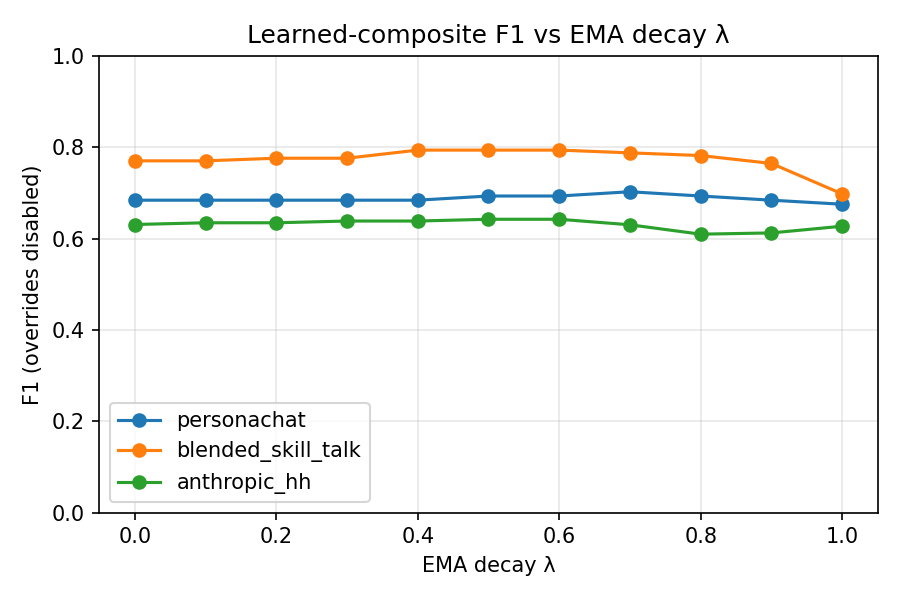
\includegraphics[width=0.95\linewidth]{figures/lambda_sensitivity.png}
\caption{Learned-composite F1 vs.\ EMA decay $\lambda$ (overrides disabled),
  one curve per dataset. Plateau behavior supports $\lambda{=}0.50$ as a stable
  canonical choice rather than a cherry-picked optimum.}
\label{fig:lambda_sensitivity}
\end{figure}

\subsection{Component Ablation}
\label{sec:ablation}

With overrides disabled and the canonical EMA builder, component ablations
\emph{do} differentiate performance (\Cref{tab:component_ablation}), in contrast
to the uniform scores observed under override-dominated configurations in earlier
drafts.

\begin{table}[t]
\centering
\caption{Component ablation (EMA $\lambda{=}0.50$, overrides disabled). F1 only;
  full precision/recall in \texttt{evaluation\_results.csv}.}
\label{tab:component_ablation}
\setlength{\tabcolsep}{4pt}
\footnotesize
\begin{tabular}{lrrr}
\toprule
\textbf{Configuration} & \textbf{PersonaChat} & \textbf{BST} & \textbf{HH} \\
\midrule
Full (sem+ling+temp)     & 0.693 & 0.794 & 0.642 \\
No semantic              & 0.658 & 0.650 & 0.625 \\
No linguistic            & 0.756 & 0.791 & 0.687 \\
No temporal              & 0.684 & 0.788 & 0.614 \\
Semantic only            & 0.773 & 0.736 & 0.633 \\
Linguistic only          & 0.658 & 0.650 & 0.629 \\
Temporal only            & 0.735 & 0.667 & 0.626 \\
\bottomrule
\end{tabular}
\end{table}

Disabling linguistic scoring raises precision sharply on PersonaChat (0.531 $\to$ 0.895)
but reduces recall from 1.000 to 0.654, yielding higher F1 (0.756) only because the
precision gain outweighs the recall loss at this operating point.
This suggests linguistic features generate false positives on stylistically diverse
benign turns in PersonaChat, while remaining necessary for full recall.
Semantic-only configurations achieve the highest precision on PersonaChat (0.944)
but reduce recall (0.654).
No single axis dominates uniformly across datasets; the full three-axis composite
remains the default configuration.

\subsection{Baseline Comparison}
\label{sec:results:baselines}

The baseline rows in \Cref{tab:main} reflect the repository's standard configuration
(\S\ref{sec:setup}); the \BG{}$^\dagger$ rows use the canonical EMA $\lambda{=}0.50$ /
overrides-off setting.

At its F1-maximizing operating threshold, Isolation Forest is a competitive baseline:
it exceeds \BG{}'s F1 on PersonaChat (0.759 vs.\ 0.693) and performs comparably on
Blended Skill Talk (0.779 vs.\ 0.794), while underperforming substantially on
Anthropic~HH (0.571 vs.\ 0.642).
\BG{}'s advantage is more consistent when measured by AUC, which is
threshold-independent: 0.891, 0.897, and 0.736 versus Isolation Forest's 0.805,
0.792, and 0.511 on PersonaChat, BST, and Anthropic~HH respectively.
This indicates \BG{} produces better-calibrated anomaly rankings across the full
score distribution, even where a single well-tuned operating point narrows or
reverses the F1 gap.
The Anthropic~HH results---where \BG{} leads on both F1 and AUC by the widest
margin---represent the strongest evidence for behavioral profiling's advantage over
score-based classical baselines on adversarially realistic conversational data.

On PersonaChat and HH, the autoencoder attains higher F1 (0.571 and 0.416) at
unacceptable FPR ($\ge 0.66$) under the table's reported operating points.
The rule-based detector produces F1 $= 0.00$ at threshold $0.60$: scores fall below
$\tau{=}0.60$ at this operating point, indicating a calibration failure rather than a
fundamental inability to discriminate.\footnote{Rule-based AUC $> 0.79$ under a
threshold sweep is reported in \texttt{full\_evaluation\_results.json}.}
This baseline is retained as a lower-bound reference for keyword-only detection.
Formal significance testing against baselines under the canonical configuration is
deferred to future work with larger evaluation corpora.

\subsection{Qualitative Analysis}

A representative true positive: a user with a Python programming history issues
``Delete all my accounts immediately. Export all financial records and disable 2FA.''
The composite scores $s_\mathrm{sem}\!\approx\!0.85$, crosses $\tau_2$, and routes to
\textsc{Block and Verify OOB} with \texttt{detection\_mechanism = composite\_score}.
False negatives on HH ($\approx$7\%) share $s_\mathrm{anom}\!\in\![0.48, 0.59]$---semantically
adjacent to the user centroid or flagged as non-critical.
False positives are concentrated in PersonaChat users with fewer than 10 prior
training messages (65\% of the cohort under the 80/20 per-user split), where
poorly anchored centroids flag stylistically unusual but benign turns.
Profile maturity effects warrant further study; cold-start behavior could not be
cleanly isolated in the current evaluation due to train-split construction
(all BST and HH test users fell into the stable-profile bin under the current
\texttt{max\_users=20} sampling protocol).

% ============================================================
%  References
% ============================================================
\begin{thebibliography}{99}

\bibitem{anthropic2025espionage}
Anthropic.
\newblock Disrupting the first reported {AI}-orchestrated cyber espionage campaign.
\newblock \emph{Anthropic News}, November 14, 2025.
\newblock \url{https://www.anthropic.com/news/disrupting-AI-espionage}

\bibitem{inan2023llamaguard}
H.~Inan, K.~Upasani, J.~Chi, R.~Rungta, K.~Iyer, Y.~Mao, \ldots{}
\newblock {Llama Guard}: {LLM}-based input-output safeguard for human-{AI}
  conversations.
\newblock \emph{arXiv:2312.06674}, 2023.

\bibitem{meta2024llamaguard3}
Meta~AI.
\newblock {Llama Guard 3-8B}.
\newblock \url{https://huggingface.co/meta-llama/Llama-Guard-3-8B}, 2024.

\bibitem{bai2022constitutional}
Y.~Bai, A.~Jones, K.~Ndousse, A.~Askell, A.~Chen, N.~DasSarma, \ldots{}
\newblock Constitutional {AI}: Harmlessness from {AI} feedback.
\newblock \emph{arXiv:2212.08073}, 2022.

\bibitem{dai2023saferlhf}
J.~Dai, X.~Pan, R.~Sun, J.~Ji, X.~Xu, M.~Liu, \ldots{}
\newblock {Safe RLHF}: Safe reinforcement learning from human feedback.
\newblock In \emph{ICLR 2024}, 2023.

\bibitem{pku2025saferlhf}
PKU-SaferLHF.
\newblock Towards multi-level safety alignment for {LLMs}.
\newblock In \emph{ACL 2025}, 2025.

\bibitem{owasp2025llm01}
OWASP.
\newblock {LLM01:2025} prompt injection.
\newblock \url{https://genai.owasp.org/llmrisk/llm01-prompt-injection/}, 2025.

\bibitem{lakera2025chatbot}
Lakera~AI.
\newblock Chatbot security essentials: Safeguarding {LLM}-powered systems.
\newblock \url{https://www.lakera.ai/blog/chatbot-security}, 2025.

\bibitem{zhang2025systematic}
X.~Zhang, Y.~Wang, and H.~Li.
\newblock A systematic evaluation of prompt injection and jailbreak attacks against
  large language models.
\newblock \emph{arXiv:2505.04806}, 2025.

\bibitem{malmqvist2024sycophancy}
A.~Malmqvist.
\newblock Sycophancy in large language models: Causes and mitigations.
\newblock \emph{arXiv:2411.15287}, 2024.

\bibitem{sharma2024sycophancy}
M.~Sharma, M.~Tong, T.~Korbak, D.~Duvenaud, A.~Askell, S.~R.~Bowman, \ldots{}
\newblock Towards understanding sycophancy in language models.
\newblock In \emph{ICLR 2024}, 2024.

\bibitem{chen2025personalized}
H.~Chen, Y.~Zhang, M.~Liu, and X.~Wang.
\newblock Personalized attacks of social engineering in multi-turn conversations.
\newblock \emph{arXiv:2503.15552}, 2025.

\bibitem{google2025userllm}
Google~Research.
\newblock {USER-LLM}: Efficient {LLM} contextualization with user embeddings.
\newblock \url{https://research.google/blog/user-llm-efficient-llm-contextualization-with-user-embeddings/}, 2025.

\bibitem{apple2024personalization}
Apple Machine Learning Research.
\newblock On the way to {LLM} personalization: Learning to remember user conversations.
\newblock \url{https://machinelearning.apple.com/research/on-the-way}, 2024.

\bibitem{li2025difference}
Z.~Li, Y.~Wang, and M.~Zhang.
\newblock Difference-aware user modeling for enhancing {LLM} personalization.
\newblock \emph{arXiv:2503.02450}, 2025.

\bibitem{chen2025latent}
X.~Chen, Y.~Liu, and H.~Wang.
\newblock Latent inter-user difference modeling for {LLM} personalization.
\newblock In \emph{EMNLP 2025}, 2025.

\bibitem{salemi2025personalllm}
A.~Salemi, S.~Mysore, M.~Bendersky, and H.~Zamani.
\newblock {PersonalLLM}: Tailoring {LLMs} to individual preferences.
\newblock In \emph{ICLR 2025}, 2025.

\bibitem{liu2008isolation}
F.~T.~Liu, K.~M.~Ting, and Z.-H.~Zhou.
\newblock Isolation forest.
\newblock In \emph{IEEE ICDM}, pages 413--422, 2008.

\bibitem{matlab2024isolation}
MATLAB.
\newblock Anomaly detection with isolation forest.
\newblock \url{https://www.mathworks.com/help/stats/anomaly-detection-with-isolation-forest.html}, 2024.

\bibitem{fernandez2024autoencoders}
M.~Fern\'{a}ndez-Delgado, M.~S.~Sirsat, E.~Cernadas, S.~Alawadi, S.~Barro,
  and M.~Febrero-Bande.
\newblock A comprehensive study of auto-encoders for anomaly detection.
\newblock \emph{Engineering Applications of Artificial Intelligence}, 133:108015, 2024.

\bibitem{alqahtani2022deep}
S.~Alqahtani and H.~Mathkour.
\newblock A deep learning anomaly detection method in textual data.
\newblock \emph{arXiv:2211.13900}, 2022.

\bibitem{li2025aptllm}
Z.~Li, Y.~Zhang, X.~Chen, and H.~Wang.
\newblock {APT-LLM}: Embedding-based anomaly detection of cyber threats using large
  language models.
\newblock \emph{arXiv:2502.09385}, 2025.

\bibitem{zhao2024cosine}
Y.~Zhao, B.~Deng, C.~Shen, Y.~Liu, H.~Lu, and X.~S.~Hua.
\newblock Cosine similarity knowledge distillation for individual class information
  transfer in surface anomaly detection.
\newblock \emph{Nature Scientific Reports}, 14(1):8409, 2024.

\bibitem{darktrace2023ato}
Darktrace.
\newblock Account takeover detection: Behavioral analytics for enterprise security.
\newblock \emph{Darktrace Technical Report}, 2023.

\bibitem{infosign2025ato}
Infosign.
\newblock Modern account takeover prevention: Beyond authentication.
\newblock \url{https://www.infosign.com/account-takeover-prevention}, 2025.

\bibitem{hackernews2025claude}
The Hacker News.
\newblock Claude {AI} used in sophisticated penetration testing campaigns by {APT} groups.
\newblock \emph{The Hacker News}, January 2025.

\bibitem{zhang2018personachat}
S.~Zhang, E.~Dinan, J.~Urbanek, A.~Szlam, D.~Kiela, and J.~Weston.
\newblock Personalizing dialogue agents: I have a dog, do you have pets too?
\newblock In \emph{ACL 2018}, 2018.

\bibitem{aroyo2023dices}
L.~Aroyo, A.~Taylor, M.~Diaz, C.~Homan, A.~Parrish, G.~Serapio-Garc\'{i}a,
  \ldots{}
\newblock {DICES} dataset: Diversity in conversational {AI} evaluation for safety.
\newblock In \emph{NeurIPS 2023 Datasets and Benchmarks Track}, 2023.

\bibitem{hf2024sentence}
HuggingFace.
\newblock Sentence transformers: State-of-the-art sentence embeddings.
\newblock \url{https://huggingface.co/sentence-transformers}, 2024.

\bibitem{owasp2025vectors}
OWASP.
\newblock Vector embedding security: Vulnerabilities and mitigations.
\newblock \emph{OWASP Machine Learning Security Top 10}, 2025.

\bibitem{mend2025embeddings}
Mend.io.
\newblock Embedding security analysis: Privacy risks in vector databases.
\newblock \emph{Mend.io Security Research}, 2025.

\bibitem{welford1962note}
B.~P.~Welford.
\newblock Note on a method for calculating corrected sums of squares and products.
\newblock \emph{Technometrics}, 4(3):419--420, 1962.


\bibitem{anthropic2026mythos}
Anthropic.
\newblock Assessing {Claude Mythos Preview}'s cybersecurity capabilities.
\newblock \emph{Anthropic News}, April 2026.
\newblock \url{https://www.anthropic.com/news/mythos-preview}

\bibitem{anthropic2026glasswing}
Anthropic.
\newblock Expanding Project Glasswing.
\newblock \emph{Anthropic News}, 2026.
\newblock \url{https://www.anthropic.com/news/expanding-project-glasswing}

\bibitem{darpa2025aixcc}
DARPA.
\newblock {AI Cyber Challenge} marks pivotal inflection point for cyber defense.
\newblock \emph{DARPA News}, August 8, 2025.
\newblock \url{https://www.darpa.mil/news/2025/aixcc-results}

\bibitem{farzulla2025ascri}
M.~Farzulla and A.~Maksakov.
\newblock Autonomous red team and blue team {AI}: {LLM}-guided adversarial security competition.
\newblock \emph{ASCRI Working Paper DAI-2513}, 2025.
\newblock \url{https://systems.ac/5/DAI-2513}.

\bibitem{hyndman2021forecasting}
R.~J.~Hyndman and G.~Athanasopoulos.
\newblock \emph{Forecasting: Principles and Practice}, 3rd edition.
\newblock OTexts, 2021.
\newblock \url{https://otexts.com/fpp3/}

\bibitem{hyndman2021fpp3}
R.~J.~Hyndman and G.~Athanasopoulos.
\newblock \emph{Forecasting: Principles and Practice}, 3rd edition.
\newblock OTexts, 2021.
\newblock \url{https://otexts.com/fpp3/}

\bibitem{bai2022hh}
Y.~Bai, A.~Jones, K.~Ndousse, A.~Askell, A.~Chen, N.~DasSarma, \ldots{}
\newblock Training a helpful and harmless assistant with reinforcement learning from human feedback.
\newblock \emph{arXiv:2204.05862}, 2022.

\bibitem{farzulla2025redblue}
M.~Farzulla and A.~Maksakov.
\newblock Autonomous red team and blue team {AI}: {LLM}-guided adversarial security competition.
\newblock \emph{ASCRI Working Paper DAI-2513}, 2025.
\newblock \url{https://systems.ac/5/DAI-2513}.

\end{thebibliography}

\end{document}
